\documentclass[12pt]{article}  
%%Read the manual for other options. 

\pagestyle{empty} %%Eliminates page numbers
%%\input rmb_macros
%%Collect your favorite macros in a 
%%separate file

%\input amssym.def
%\input amssym
%\input mssymb
%%Defines additional symbols



\usepackage{graphics}
\usepackage{amsmath,amssymb,amsthm, multicol}
\usepackage[pdftex]{graphicx}
\usepackage{epsf}
%%Use to include pictures. 

%\newcommand{\comment}[1]{}
%\newcommand{\sobolev}[2]{W^{#1,#2}}
%\newcommand{\sobolev}[2]{L^#2_#1}
%%Some examples of macros or new commands.

\addtolength{\oddsidemargin}{-.75in}
\addtolength{\evensidemargin}{-.75in}
\addtolength{\textwidth}{1.5in}
\addtolength{\topmargin}{-1in}
\addtolength{\textheight}{2.25in}
%%Set margins, defaults are ok. 

\newcommand{\integers}{\mathbb{Z}}

\begin{document}
\begin{center}
{\bf \Large Secret Sharing}
\vspace{0.2cm}
\hrule
\end{center}

\section*{What is Secret Sharing?}
The goal of secret sharing is dividing a secret $S$ into $n$ pieces (or \textit{shares}) so that no fewer than $k\leq n$ pieces are sufficient for reassembling $S$. This is called a $(k,n)$-threshold scheme.

\section*{Why is Secret Sharing?}
As Shamir puts it, ``Threshold schemes are ideally suited to applications in which a group of mutually suspicious individuals with conflicting interests must cooperate.''\\

%\noindent Here's an example. Say a company signs its checks. If any one executive could sign off on a check, then this system could be easily abused by just one rogue executive. Suppose the moderately-sized company has $n$ executives. We can set up a $(3, n)$-threshold system where each executive is issued a card containing a share of the company's signing key. If an executive wants to sign a check, they have to place their check into a check-signing device. Then they and two other executives swipe their cards at the machine. The machine then temporarily generates the company's signature key and signs the check. Now a rogue employee needs at least two accomplices to sign malicious checks.
Some uses include flexibly enforcing consensus while granting veto power and allowing for packets to be sent over a network securely and efficiently.


\section*{How is Secret Sharing?}
\subsection*{Shamir's Secret Sharing (1979)\footnote{A. Shamir, ``How to share a secret''. Commun. ACM 22(11), 612–613 (1979)}}
Shamir's approach is based on polynomial interpolation. Say we want to share a secret among $n$ people so that no fewer than $k$ of them can recover the secret. Choose a big prime $p$ and say our secret is an element $S\in \integers/p\integers$. Choose random elements $a_1,\ \ldots, a_{k-1}\in \integers/p\integers$ and set
\[
p(x) = S + a_1x + \cdots + a_{k-1}x^{k-1}.
\]

\noindent Issue to person $i$ the share $D_i = (i, p(i))$, $1\leq i\leq n$. If $m$ people come together with their shares, $(i_j, p(i_j))$, $1\leq j\leq m$ then they know that
\[
\begin{array}{ccccccccccc}
	S & + & a_1\cdot i_1 & + & a_2\cdot (i_1)^2 &+& \cdots& + & a_{k-1}(i_1)^{k-1} & = & p(i_1)\\
	S & + & a_2\cdot i_2 & + & a_2\cdot (i_2)^2 &+& \cdots& + & a_{k-1}(i_2)^{k-1} & = & p(i_2)\\
	&&&&&&\vdots&&&\\
	S & + & a_1\cdot i_m & + & a_2\cdot (i_m)^2 &+& \cdots& + & a_{k-1}(i_m)^{k-1} & = & p(i_m)
\end{array}
\]
This represents a system of $m$ equations in the $k$ unknowns, $S$, $a_1$, $\ldots$, $a_{k-1}$. Elementary linear algebra tells us that this system has a unique solution if and only if $m\geq k$. That is, we need at least $k$ shares in order to uniquely determine $S$.

\subsection*{Main Disadvantage of Shamir's Scheme}
Each share is just as large as the secret. $n$ shares means $n$-fold blowup in storage.

\section*{Improvements by Rabin and Krawczyk}
\subsection*{Rabin - Information Dispersal (1989)\footnote{M. O. Rabin, ``Efficient Dispersal of Information for Security, Load Balancing, and Fault Tolerance''. In: Journal of the ACM, vol. 36, iss. 2, 1989, pp. 335-348}}
We can split a file $F$ into $n$ pieces so that any $k\leq n$ pieces are sufficient for reconstructing $F$, with the added feature that each piece has size roughly $|F|/k$. With $n$ shares, each of size roughly $|F|/k$ we get a blowup of around $\frac{n}{k}$, but this can be chosen to be close to 1. \textit{Secrecy isn't the objective.}\\

% \noindent Say the file $F$ is composed of bytes, $F = b_1, b_2, \ldots, b_N$, where each $b_i$ is an integer $0\leq b_i\leq 255$. Let $p$ be a prime bigger than $255$, such as $p = 257$. Choose $n$ vectors, $a_i = (a_{i1}, \ldots, a_{im})$, $1\leq i\leq n$, in $(\integers/p\integers)^m$ so that any subset of $m$ different vectors is linearly independent (how this can be done is a non-obvious but still elementary exercise in linear algebra). Break the file into blocks of length $m$,
% \[
% F = (b_1, \ldots, b_m), (b_{m+1}, \ldots, b_{2m}), \ldots = f_1, f_2, \ldots,
% \]
%  where $f_1 = (b_1, \ldots, b_m)$ is the first block of $F$, and so on. We set the $i$-th share to be $S_i = (a_i, F_i)$, $1\leq i\leq n$ where
%  \[
%  F_i = c_{i1}, \ldots, c_{iN/m},
%  \]
%  and
%  \[
%  c_{ik} = a_i\cdot f_k = a_{i1}\cdot b_{(k-1)m+1} + \cdots +a_{im}\cdot b_{km}.
%  \]
%  Each share has length $|a_i| + |F_i| = m + \frac{|F|}{m}$. Now say we're given $m$ shares, $(a_1, F_1), \ldots, (a_m, F_m)$. We can reconstruct $F$ as follows. Let $A$ be the matrix whose rows are $a_i$, $1\leq i\leq m$. Then by construction we have for $1\leq j\leq m$
%  \[
%  A f_1 = A\begin{bmatrix}
%  	b_1\\
%  	\vdots\\
%  	b_m
%  \end{bmatrix} = \begin{bmatrix}
%  	c_{11}\\
%  	\vdots\\
%  	c_{m1}
%  \end{bmatrix} = F_1.
%  \]
%  Since the rows of $A$ are designed to be linearly independent, we can invert the above equation to obtain
%  \[
%  f_1 = \begin{bmatrix}
%  	b_1\\
%  	\vdots\\
%  	b_m
%  \end{bmatrix} = A^{-1} F_1.
%  \]

\noindent Say the file $F$ is composed of bytes, $F = b_1, \ldots, b_N$, where each $b_i$ is an integer $0\leq b_i\leq 255$. Let $p$ be a prime bigger than 255. Break the file into $k$-byte blocks
\[
F = (b_1, \ldots, b_k), (b_{k+1}, \ldots, b_{2k}), \ldots = f_1, f_2, \ldots, f_{N/m}
\]
where $f_1 = (b_1, \ldots, b_k)$ is the first block, and so on. The idea is to compress each $k$-byte block into a single number in such a way that any $k$ compressed blocks can be used to recover the original block.\\

\noindent To create $n$ shares, choose $n$ vectors, $a_j$ in $(\integers/p\integers)^m$ so that any subset of $m$ different vectors is linearly independent (how this can be done is a non-obvious, but still elementary exercise in linear algebra). To compute the $j$-th share, we compress each block of the file by calculating the dot product $F_{ji} = a_j\cdot f_i\pmod{p}$ for each $1\leq i\leq N/m$.

\begin{figure}[h]
 	\centering
 		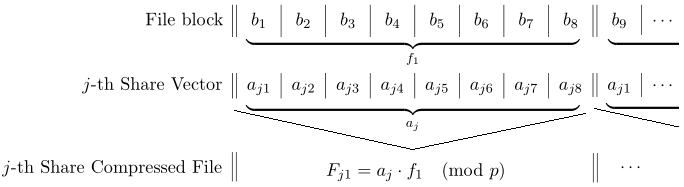
\includegraphics[scale=.7]{rabin_compression.png}
 	\caption{Compressing $F$ into a share.}
\end{figure} 

\subsection*{Krawczyk - Secret Sharing with Short Shares (1994)\footnote{H. Krawczyk, ``Secret Sharing Made Short''. In: Stinson D.R. (eds) Advances in Cryptology — CRYPTO’ 93. CRYPTO 1993. Lecture Notes in Computer Science, vol 773.}}
Combine the ideas of Shamir and Rabin. We want to set up a $(k,n)$ threshold scheme with secret $S$. We start by encrypting $S$ with some secure cipher using key $K$, $E = Enc(S, K)$. Using Rabin's information dispersal method, partition $E$ into $n$ shares, $E_1, \ldots, E_n$ so that any $k$ of them can rebuild $E$. Using Shamir's method, generate $n$ shares of the key, $K_1, \ldots, K_n$ so that any $k$ of them can rebuild $K$. Send person $i$ the pair $(E_i, K_i)$.\\

\noindent Now when $k$ people come together, they can reassemble $E$ through Rabin's matrix inversion method and $K$ through polynomial interpolation. The $k$ participants can then decrypt $E$ with $K$ to obtain $S$.\\

\noindent While Shamir's method didn't shrink the size of the key shares, Rabin's method shrinks the size of the secret shares.



% k people
% k-1 degree
% k-1 

\end{document}